\documentclass[12pt, a4paper]{article}
\usepackage[margin=1.25in]{geometry}
\usepackage{graphicx}
\usepackage{amsmath}
\usepackage{float}
\usepackage{listings}
\usepackage{caption}
\usepackage{physics}
\usepackage[shortlabels]{enumitem}


\setlength\parindent{0pt}
\newcommand{\code}{\lstinline[basicstyle=\small]}
\lstset{
    language=Python,
    basicstyle=\scriptsize
}


\title{EE2703: Applied Programming Lab \\ \Large Assignment 6: The Laplace Transform}
\author{Soham Roy \\ \normalsize EE20B130}
\date{\today}
\begin{document}

\maketitle % Insert the title, author and date



\section{Introduction}
The goals of this assignment are:
\begin{itemize}
    \item To analyze LTI Systems using Laplace Transform.
    \item To see how RLC systems can be used as a low pass filter.
    \item To understand how to use the \code{scipy.signals} toolkit.
    \item To plot graphs to understand the Laplace Transform.
\end{itemize}




\section{Subquestions}
\subsection{Time Response of a Spring}
We use the Laplace transform to solve a simple spring system.
The system is characterized by the differential equation:
\[\dv[2]{x}{t} + 2.25x = f(t)\]
with initial values being 0.
The Laplace Transform of the differential equation is:
\[H(s) =  \frac{1}{s^2+2.25}\]
The input signal is of the form \(f(t) = \cos{(\omega t)}\exp(-at)u(t)\),
where $a$ is the decay factor and $\omega$ is the frequency of the cosine. \\
The Laplace Transform of the input signal is:
\[ F(s) = \frac{s+a}{(s+a)^2+\omega^2 }\]
First, these function are defined using numpy polynomials and multiply to get the output Laplace Transform.
Then, the ILT of the function is evaluated using \code{sp.impulse} to get the time domain sequences.
This is done for $\omega=1.5$ (natural frequency of the system), and decay of 0.5.
\pagebreak

The time response is evaluated using:
\begin{lstlisting}
    def time_response_spring(decay):
        den = np.polymul([1, 0, 1.5**2], [1, 2*decay, decay**2 + 1.5**2])
        return sp.lti([1, decay], den)
\end{lstlisting}

The impulse response is then plotted using:
\begin{lstlisting}
    t, x = sp.impulse(time_response_spring(0.5), T=np.linspace(0, 50, 501))
    plot(t, x, "Damped Oscillator with 0.5/s Decay", "$t$", "$x$")
\end{lstlisting}

Thus, we get:
\begin{figure}[H]
    \centering
    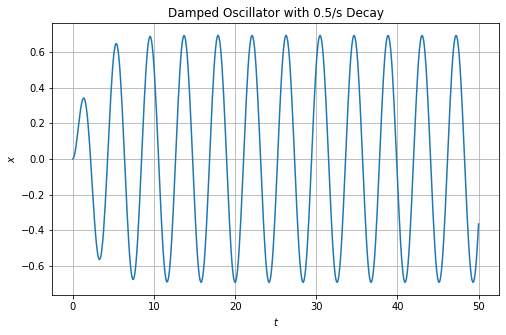
\includegraphics[scale=0.6]{1.png}
\end{figure}


\subsection{Time Response with a Smaller Decay}
We do the same for a decay of 0.05. The impulse response is then plotted using:
\begin{lstlisting}
    _, x = sp.impulse(time_response_spring(0.05), T=t)
    plot(t, x, "Damped Oscillator with 0.05/s Decay", "$t$", "$x$")
\end{lstlisting}

Thus, we get:
\begin{figure}[H]
    \centering
    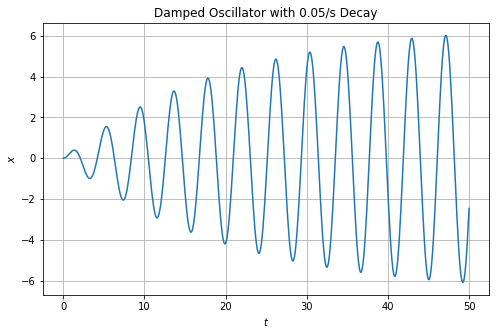
\includegraphics[scale=0.6]{2.png}
\end{figure}


\subsection{Time Response at Varying Frequencies}
The frequency of the cosine term in $f(t)$ is varied from 1.4 to 1.6 in steps of 0.05
and its effect plotted using:
\begin{lstlisting}
    H = sp.lti([1], [1, 0, 1.5 ** 2])

    for i, freq in enumerate(np.linspace(1.4, 1.6, 5)):
        f = np.cos(freq * t) * np.exp(-0.05 * t) * (t >= 0)
        x = sp.lsim(H, f, t)[1]
        plt.plot(t, x)
\end{lstlisting}
\begin{figure}[H]
    \centering
    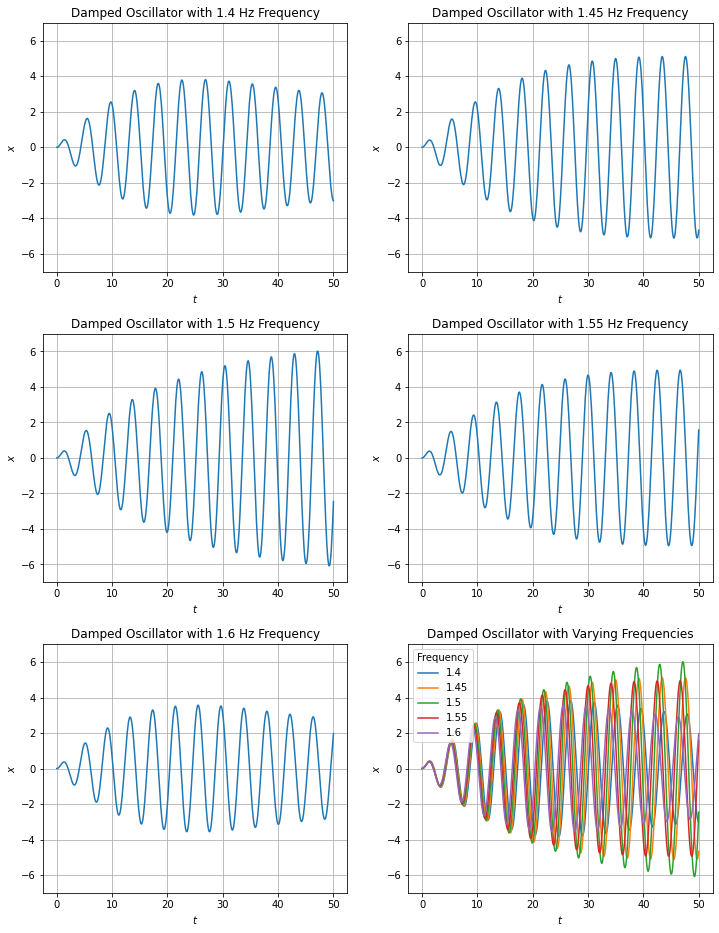
\includegraphics[scale=0.55]{3.png}
\end{figure}

When the input frequency is at the natural frequency, the output amplitude is maximum.
In the other cases the output amplitude decreases. \\
This is due to resonance.


\subsection{Coupled Spring Problem}
In this problem we have two differential equations and two variables to solve for.
The equations are:
\[\dv[2]{x}{t} +(x-y) = 0 \]
\[\dv[2]{y}{t} +2(y-x) = 0 \]
with initial condition as $x(0) = 1$. $y$ in the second equation is substituted from the first,
and a fourth order differential equation in terms of $x$ is obtained.
Simplifying this results in:
\[X(s) = \frac{s^2+2}{s^3+3s} \]
\[Y(s) =  \frac{2}{s^3+3s} \]
Taking the ILT of these two expressions gives the time domain expressions of $x(t)$ and $y(t)$:
\begin{lstlisting}
    # d2x/dt2 + (x - y) = 0
    # d2y/dt2 + 2*(y - x) = 0
    t, x = sp.impulse(sp.lti([1, 0, 2], [1, 0, 3, 0]), T=np.linspace(0, 20, 201))
    _, y = sp.impulse(sp.lti([2], [1, 0, 3, 0]), T=t)

    plot(t, x)
    plot(t, y, "Coupled Springs", "t", "$x(t)$  &  $y(t)$", ["$x(t)$", "$y(t)$"])
\end{lstlisting}
These have been plotted as functions of time:
\begin{figure}[H]
    \centering
    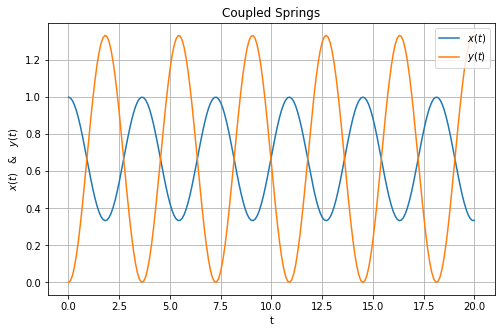
\includegraphics[scale=0.6]{4.png}
\end{figure}


\subsection{Magnitude \& Phase Responses of Transfer Function}
The transfer function of the given RLC filter is:
\[ H(s) = \frac{1}{LCs^2 + RCs + 1}\]
with the initial conditions being zero. This is evaluated using:
\begin{lstlisting}
    H = sp.lti([1], [1e-6 * 1e-6, 100 * 1e-6, 1])
\end{lstlisting}
The magnitude and phase responses of the transfer function are plotted using:
\begin{lstlisting}
    w, S, phi = H.bode()
    plt.semilogx(w, S)
    plt.semilogx(w, phi)
\end{lstlisting}
\begin{figure}[H]
    \centering
    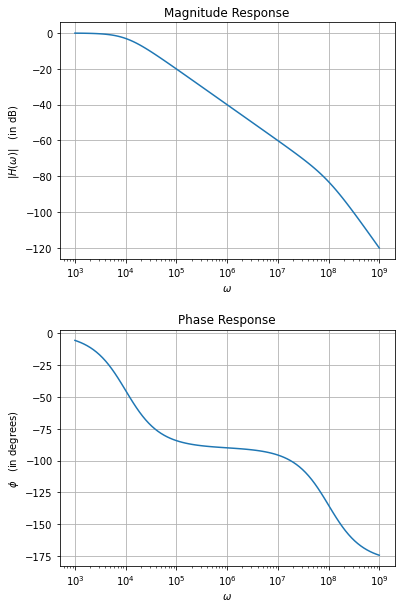
\includegraphics[scale=0.6]{5.png}
\end{figure}

From the Bode plots, it is clear that the RLC System is a second order low pass filter,
with a 3db bandwidth of $10^4$ rad/s.
\pagebreak


\subsection{Analysis of the Output Signal}
The input is of the form:
\[v_i(t) = \cos{(10^3t)}u(t) - \cos{(10^6t)}u(t)\]
The output voltage $v_o(t)$ is obtained by:
\begin{lstlisting}
    def v_o(t, H):
        v_i = np.cos(1e3 * t) * (t >= 0) - np.cos(1e6 * t) * (t >= 0)
        return sp.lsim(H, v_i, t)[1]
\end{lstlisting}

The output voltage is then plotted using:
\begin{lstlisting}
    y = v_o(np.linspace(0, 30e-6, 10000), H)
    plot(np.linspace(0, 30, 10000), y,
         "Output Voltage for $0<t<30\mu$s (short term)",
         "$t$ (in $\mu$s)", "$V_o(t)$")

    y = v_o(np.linspace(0, 15e-3, 10000), H)
    plot(np.linspace(0, 15, 10000), y,
         "Output Voltage for $0<t<15m$s (long term)", "$t$ (in ms)", "$V_o(t)$")
\end{lstlisting}
\begin{figure}[H]
    \centering
    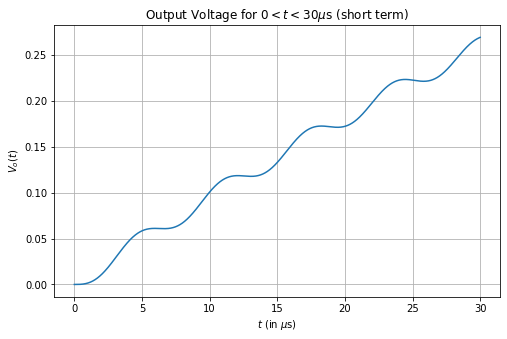
\includegraphics[scale=0.6]{6a.png}
\end{figure}
\begin{figure}[H]
    \centering
    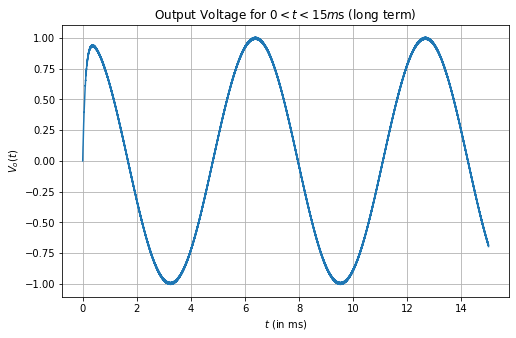
\includegraphics[scale=0.6]{6b.png}
\end{figure}

From the Bode plot, it is clear that the RLC System is a second order low pass filter,
with a 3db bandwidth of $10^4$ rad/s. \\
The short term response plot shows that the capacitor is charging up to meet the input amplitude. \\
The high frequency component can be seen as a ripple in the short term response plot.
This component is highly attenuated and hence not visible in the long term response plot. \\
In the long term response plot, the low frequency component passes almost unchanged,
and the amplitude is almost 1. This is because $\omega = 10^3$ rad/s is well within the 3-dB bandwidth
($\omega_{3dB} = 10^4$ rad/s) of the system. \\
Clearly, this demonstrates the fact that this is a low pass filter with bandwidth
$\omega_{3dB} = 10^4$ rad/s.



\section{Conclusion}
\begin{itemize}
    \item We analyzed LTI Systems using the Laplace Transform.
    \item We saw a low pass filter constructed from an RLC circuit.
    \item We used the scipy signals toolkit to calculate the time domain response and the Bode Plot.
    \item We plotted graphs to understand the above.
\end{itemize}



\end{document}
